\documentclass[12pt,a4paper]{article}

% --- Encodage & langue ---
\usepackage[T1]{fontenc}
\usepackage[utf8]{inputenc}
\usepackage[french]{babel}
\usepackage{lmodern}

% --- Mise en page --
\usepackage{geometry}
\geometry{margin=2.2cm}
\pagestyle{empty}

% --- Images ---
\usepackage{graphicx}
\graphicspath{{images/}}

% --- Flèches / annotations ---
\usepackage{tikz}
\usetikzlibrary{arrows.meta}

\begin{document}

\begin{center}
\begin{tikzpicture}[>=Latex]

  % Taille des vignettes (ajuste 0.20 -> 0.16/0.22 selon goût)
  \def\w{0.20\textwidth}

  % --- 4 photos (2x2) ---
  \node[inner sep=0pt] (p1) at (-4,  3) {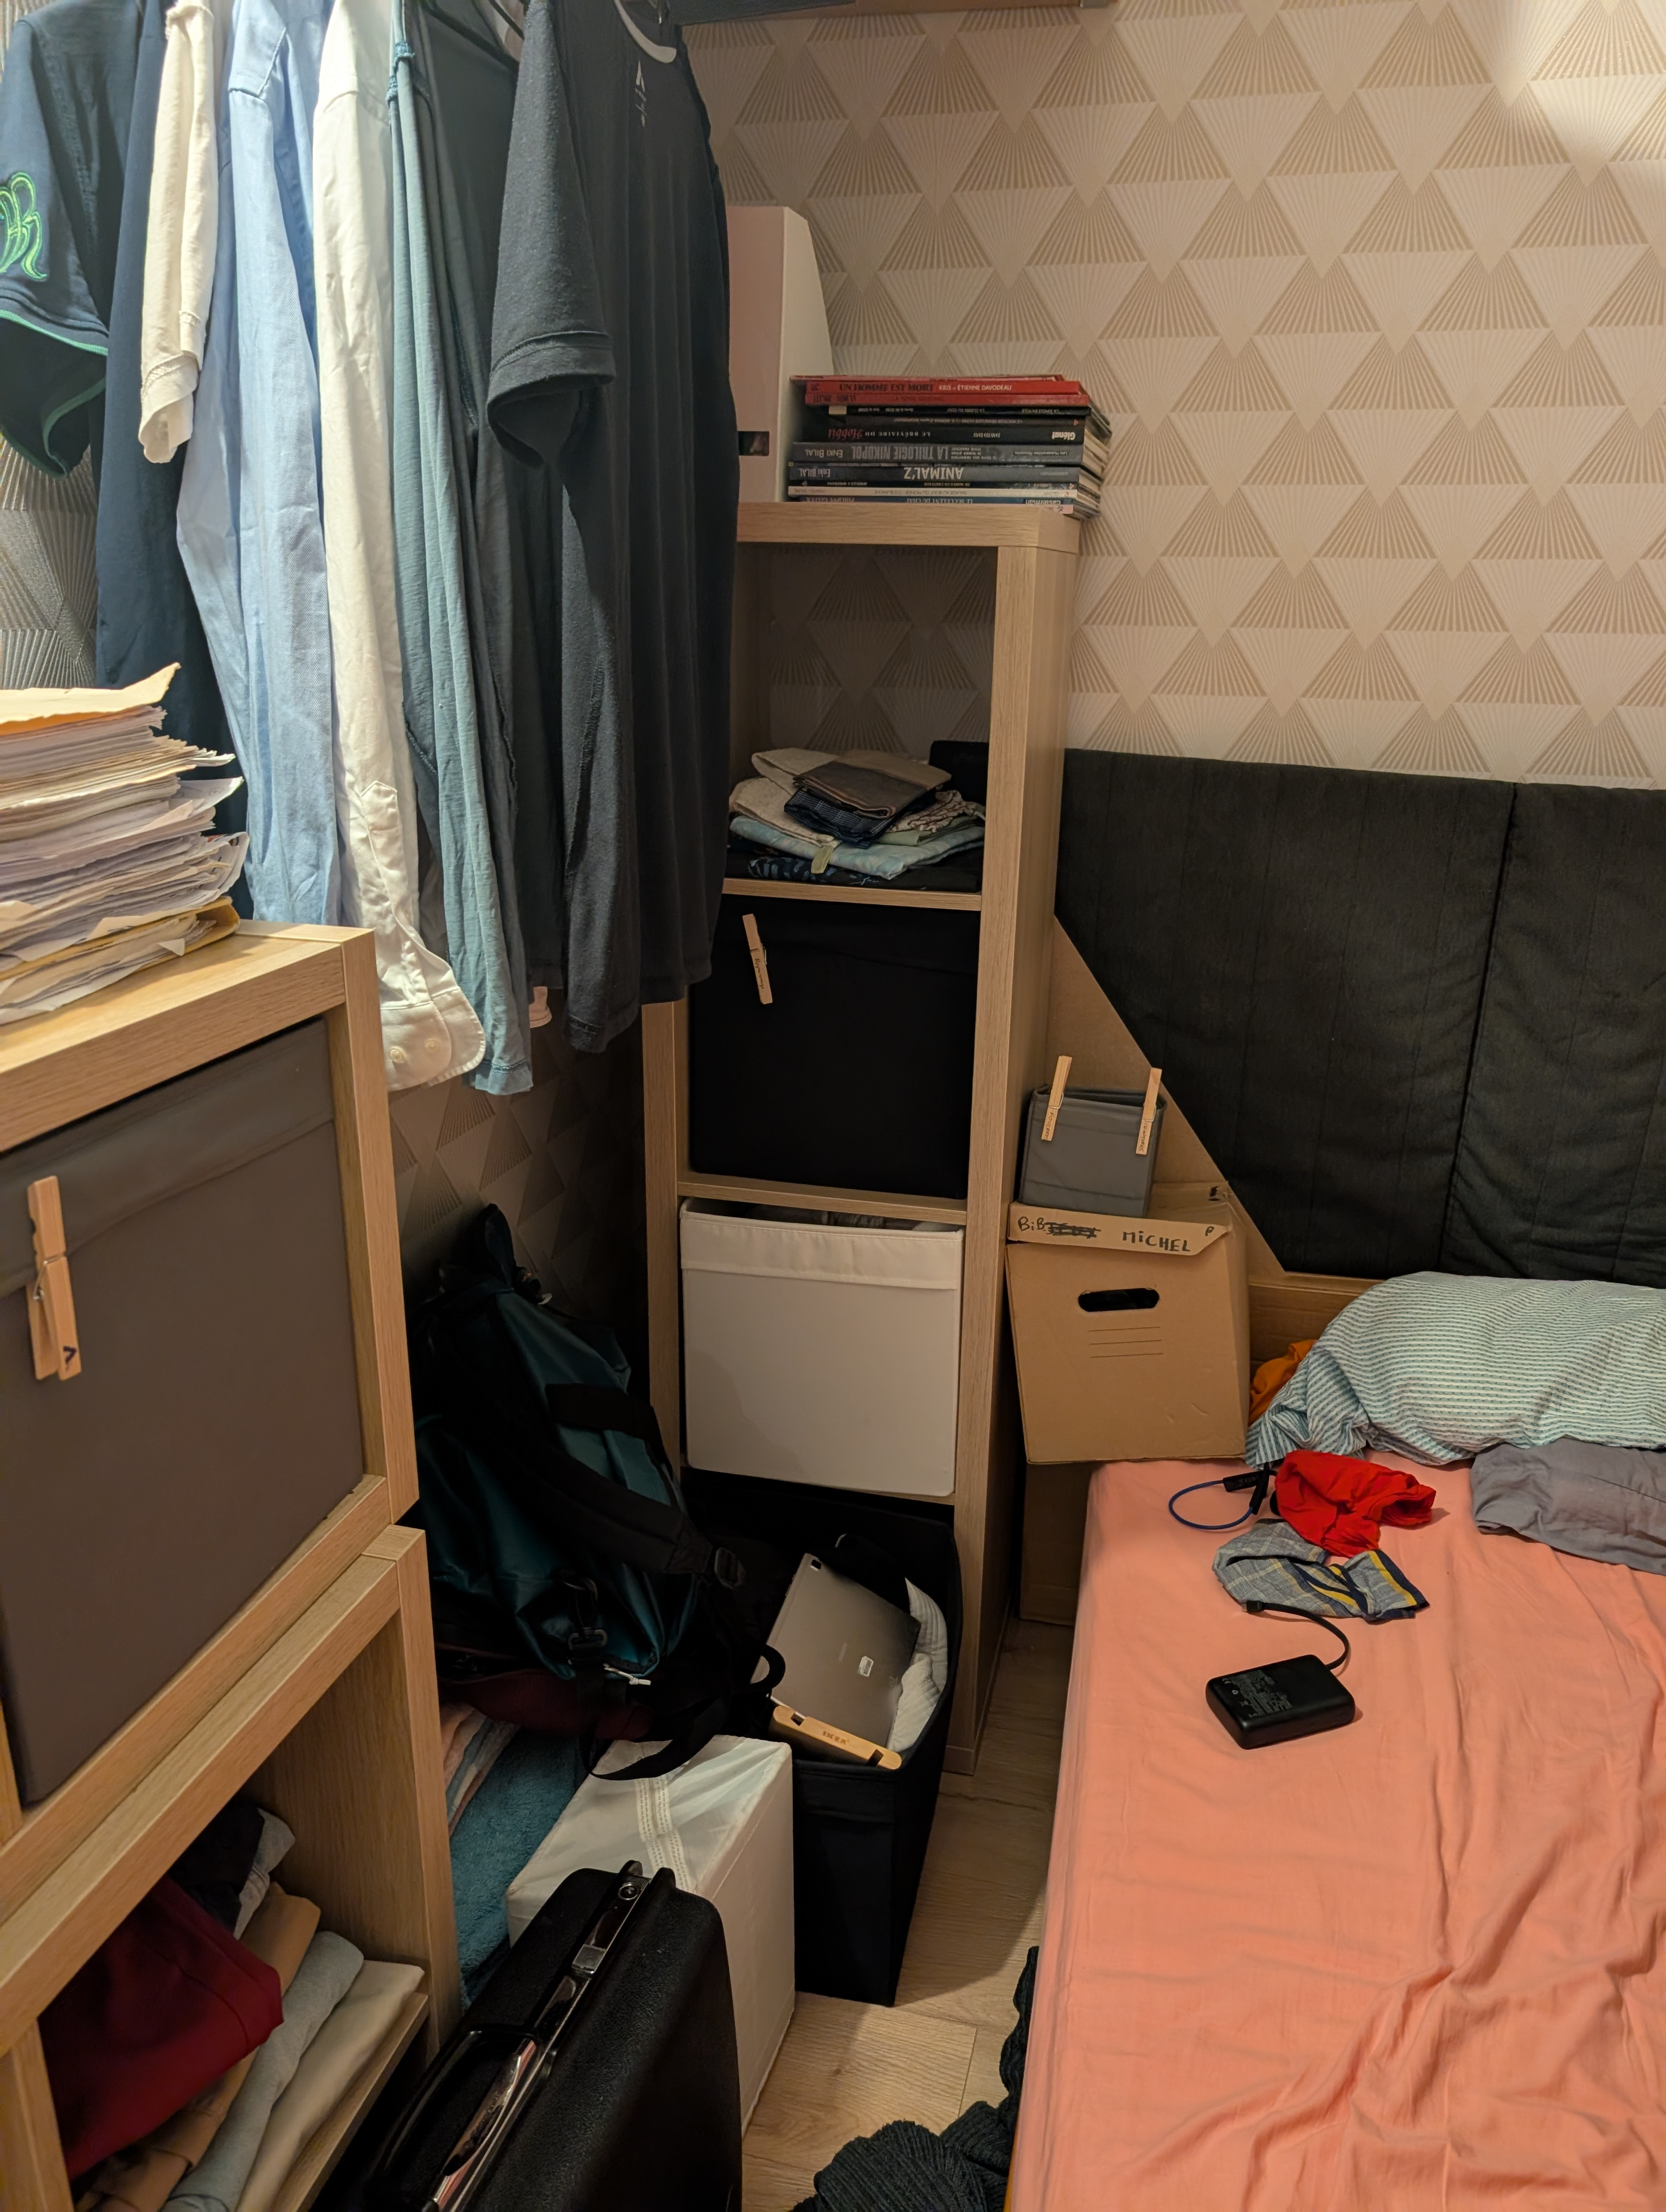
\includegraphics[width=\w]{photo1.jpg}};
  \node[inner sep=0pt] (p2) at ( 4,  3) {\includegraphics[width=\w]{photo2.jpg}};
  \node[inner sep=0pt] (p3) at (-4, -3) {\includegraphics[width=\w]{photo3.jpg}};
  \node[inner sep=0pt] (p4) at ( 4, -3) {\includegraphics[width=\w]{photo4.jpg}};

  % --- Commentaires + flèches (1 bloc par photo) ---

  \node[align=justify, text width=6cm] (t1) at (-9,  3) {%
  \textbf{Photo 1 — Salon}\par
  Exemple : luminosité, état des murs, détails à vérifier, etc.
};
  \draw[->] (t1.east) -- (p1.west);

  \node[align=left, text width=6cm] (t2) at ( 9,  3) {%
    \textbf{Photo 2 — Cuisine}\\
    Exemple : rangements, prises,\\
    circulation, etc.
  };
  \draw[->] (t2.west) -- (p2.east);

  \node[align=right, text width=6cm] (t3) at (-9, -3) {%
    \textbf{Photo 3 — Chambre}\\
    Exemple : sol, fenêtre,\\
    travaux éventuels.
  };
  \draw[->] (t3.east) -- (p3.west);

  \node[align=left, text width=6cm] (t4) at ( 9, -3) {%
    \textbf{Photo 4 — Salle de bain}\\
    Exemple : ventilation, joints,\\
    humidité, etc.
  };
  \draw[->] (t4.west) -- (p4.east);

\end{tikzpicture}
\end{center}

\end{document}
